\documentclass[10pt]{article}\usepackage[]{graphicx}\usepackage[]{color}
%% maxwidth is the original width if it is less than linewidth
%% otherwise use linewidth (to make sure the graphics do not exceed the margin)
\makeatletter
\def\maxwidth{ %
  \ifdim\Gin@nat@width>\linewidth
    \linewidth
  \else
    \Gin@nat@width
  \fi
}
\makeatother

\definecolor{fgcolor}{rgb}{0.345, 0.345, 0.345}
\newcommand{\hlnum}[1]{\textcolor[rgb]{0.686,0.059,0.569}{#1}}%
\newcommand{\hlstr}[1]{\textcolor[rgb]{0.192,0.494,0.8}{#1}}%
\newcommand{\hlcom}[1]{\textcolor[rgb]{0.678,0.584,0.686}{\textit{#1}}}%
\newcommand{\hlopt}[1]{\textcolor[rgb]{0,0,0}{#1}}%
\newcommand{\hlstd}[1]{\textcolor[rgb]{0.345,0.345,0.345}{#1}}%
\newcommand{\hlkwa}[1]{\textcolor[rgb]{0.161,0.373,0.58}{\textbf{#1}}}%
\newcommand{\hlkwb}[1]{\textcolor[rgb]{0.69,0.353,0.396}{#1}}%
\newcommand{\hlkwc}[1]{\textcolor[rgb]{0.333,0.667,0.333}{#1}}%
\newcommand{\hlkwd}[1]{\textcolor[rgb]{0.737,0.353,0.396}{\textbf{#1}}}%
\let\hlipl\hlkwb

\usepackage{framed}
\makeatletter
\newenvironment{kframe}{%
 \def\at@end@of@kframe{}%
 \ifinner\ifhmode%
  \def\at@end@of@kframe{\end{minipage}}%
  \begin{minipage}{\columnwidth}%
 \fi\fi%
 \def\FrameCommand##1{\hskip\@totalleftmargin \hskip-\fboxsep
 \colorbox{shadecolor}{##1}\hskip-\fboxsep
     % There is no \\@totalrightmargin, so:
     \hskip-\linewidth \hskip-\@totalleftmargin \hskip\columnwidth}%
 \MakeFramed {\advance\hsize-\width
   \@totalleftmargin\z@ \linewidth\hsize
   \@setminipage}}%
 {\par\unskip\endMakeFramed%
 \at@end@of@kframe}
\makeatother

\definecolor{shadecolor}{rgb}{.97, .97, .97}
\definecolor{messagecolor}{rgb}{0, 0, 0}
\definecolor{warningcolor}{rgb}{1, 0, 1}
\definecolor{errorcolor}{rgb}{1, 0, 0}
\newenvironment{knitrout}{}{} % an empty environment to be redefined in TeX

\usepackage{alltt}
\usepackage{amsfonts,amssymb,amsmath,amsthm,graphicx,accents,enumerate}
\usepackage[utf8]{inputenc}
\usepackage[T1]{fontenc}        
\usepackage[spanish]{babel}
\decimalpoint
\advance\hoffset by -0.9in
\advance\textwidth by 1.8in
\advance\voffset by -1in
\advance\textheight by 2in
\parskip= 1 ex
\parindent = 10pt
\baselineskip= 13pt
\newcommand{\red}[1]{\textcolor{red}{#1}}


\renewcommand{\leq}{\leqslant}
\renewcommand{\geq}{\geqslant}

\newcounter{problemes}
\newcounter{punts} \def\thepunts{\arabic{punts}}
\def\probl{\addtocounter{problemes}{1} \setcounter{punts}{0}
\medskip\noindent{\bf \theproblemes) }}
\def\punt{\addtocounter{punts}{1} \smallskip{\emph{\thepunts) }}}

\newcommand{\novapart}{\noindent\hrulefill}
\newcommand{\VV}{\textbf{\Large \checkmark}}
\newcommand{\coment}[1]{\noindent{\footnotesize\textbf{Comentario}: #1\par}}
\newcommand{\sol}[1]{{\footnotesize #1\par}}

\renewcommand{\VV}{}
\renewcommand{\sol}[1]{}
\renewcommand{\coment}[1]{}


\pagestyle{empty}
\IfFileExists{upquote.sty}{\usepackage{upquote}}{}
\begin{document}
%\SweaveOpts{concordance=TRUE}
%1
\noindent\emph{Nombre:}\hfill\hfill\hfill\hfill\hfill\hfill\hfill\ \emph{Grupo:}\hfill \vspace*{-2ex}

\begin{center}
\textsc{Matemáticas III. GMAT. Control 2 11 junio 2017-2018. Ejercicios.}
\end{center}



\setcounter{problemes}{0}
\probl El \verb+data frame+ \verb+datos_vuelos+ contiene información del retraso en minutos de vuelos de varias compañías aéreas diferentes.




\begin{knitrout}
\definecolor{shadecolor}{rgb}{0.969, 0.969, 0.969}\color{fgcolor}\begin{kframe}
\begin{alltt}
\hlkwd{head}\hlstd{(datos_vuelos)}
\end{alltt}
\begin{verbatim}
##     retraso compania
## 1  8.308064       C1
## 2  3.800487       C1
## 3  9.742283       C1
## 4 11.083525       C1
## 5 16.941135       C1
## 6  8.941155       C1
\end{verbatim}
\begin{alltt}
\hlkwd{str}\hlstd{(datos_vuelos)}
\end{alltt}
\begin{verbatim}
## 'data.frame':	250 obs. of  2 variables:
##  $ retraso : num  8.31 3.8 9.74 11.08 16.94 ...
##  $ compania: Factor w/ 5 levels "C1","C2","C3",..: 1 1 1 1 1 1 1 1 1 1 ...
\end{verbatim}
\begin{alltt}
\hlstd{anova_sol}\hlkwb{=}\hlkwd{aov}\hlstd{(retraso}\hlopt{~}\hlstd{compania,}\hlkwc{data}\hlstd{=datos_vuelos)}
\hlkwd{summary}\hlstd{(anova_sol)}
\end{alltt}
\begin{verbatim}
##              Df Sum Sq Mean Sq F value Pr(>F)    
## compania      4  25174    6293   375.5 <2e-16 ***
## Residuals   245   4106      17                   
## ---
## Signif. codes:  0 '***' 0.001 '**' 0.01 '*' 0.05 '.' 0.1 ' ' 1
\end{verbatim}
\begin{alltt}
\hlkwd{pairwise.t.test}\hlstd{(datos_vuelos}\hlopt{$}\hlstd{retraso,datos_vuelos}\hlopt{$}\hlstd{compania,}\hlstr{"none"}\hlstd{)}
\end{alltt}
\begin{verbatim}
## 
## 	Pairwise comparisons using t tests with pooled SD 
## 
## data:  datos_vuelos$retraso and datos_vuelos$compania 
## 
##    C1     C2     C3   C4  
## C2 0.32   -      -    -   
## C3 <2e-16 <2e-16 -    -   
## C4 <2e-16 <2e-16 0.52 -   
## C5 <2e-16 <2e-16 0.59 0.91
## 
## P value adjustment method: none
\end{verbatim}
\begin{alltt}
\hlkwd{library}\hlstd{(agricolae)}
\hlkwd{duncan.test}\hlstd{(anova_sol,}\hlstr{"compania"}\hlstd{,}\hlkwc{group}\hlstd{=}\hlnum{TRUE}\hlstd{)}\hlopt{$}\hlstd{groups}
\end{alltt}
\begin{verbatim}
##      retraso groups
## C4 30.766867      a
## C5 30.671788      a
## C3 30.235084      a
## C2 10.490940      b
## C1  9.678596      b
\end{verbatim}
\begin{alltt}
\hlkwd{duncan.test}\hlstd{(anova_sol,}\hlstr{"compania"}\hlstd{,}\hlkwc{group}\hlstd{=}\hlnum{FALSE}\hlstd{)}\hlopt{$}\hlstd{comparison}
\end{alltt}
\begin{verbatim}
##           difference pvalue signif.        LCL         UCL
## C1 - C2  -0.81234391 0.3221          -2.425113   0.8004253
## C1 - C3 -20.55648850 0.0000     *** -22.254224 -18.8587532
## C1 - C4 -21.08827137 0.0000     *** -22.884526 -19.2920168
## C1 - C5 -20.99319169 0.0000     *** -22.747649 -19.2387340
## C2 - C3 -19.74414459 0.0000     *** -21.356914 -18.1313754
## C2 - C4 -20.27592746 0.0000     *** -22.030385 -18.5214698
## C2 - C5 -20.18084778 0.0000     *** -21.878583 -18.4831125
## C3 - C4  -0.53178287 0.5449          -2.229518   1.1659524
## C3 - C5  -0.43670319 0.5943          -2.049472   1.1760660
## C4 - C5   0.09507968 0.9077          -1.517690   1.7078489
\end{verbatim}
\begin{alltt}
\hlkwd{library}\hlstd{(car)}
\end{alltt}


{\ttfamily\noindent\itshape\color{messagecolor}{\#\# Loading required package: carData}}\begin{alltt}
\hlkwd{leveneTest}\hlstd{(datos_vuelos}\hlopt{$}\hlstd{retraso,datos_vuelos}\hlopt{$}\hlstd{compania)}
\end{alltt}
\begin{verbatim}
## Levene's Test for Homogeneity of Variance (center = median)
##        Df F value Pr(>F)
## group   4  0.3552 0.8403
##       245
\end{verbatim}
\begin{alltt}
\hlkwd{bartlett.test}\hlstd{(datos_vuelos}\hlopt{$}\hlstd{retraso,datos_vuelos}\hlopt{$}\hlstd{compania)}
\end{alltt}
\begin{verbatim}
## 
## 	Bartlett test of homogeneity of variances
## 
## data:  datos_vuelos$retraso and datos_vuelos$compania
## Bartlett's K-squared = 0.38658, df = 4, p-value = 0.9836
\end{verbatim}
\begin{alltt}
\hlkwd{library}\hlstd{(nortest)}
\hlkwd{sapply}\hlstd{(}\hlkwd{levels}\hlstd{(datos_vuelos}\hlopt{$}\hlstd{compania),}\hlkwc{FUN}\hlstd{=}\hlkwa{function}\hlstd{(}\hlkwc{x}\hlstd{)\{}
  \hlkwd{lillie.test}\hlstd{(datos_vuelos[datos_vuelos}\hlopt{$}\hlstd{compania}\hlopt{==}\hlstd{x,}\hlstr{"retraso"}\hlstd{])\}}
  \hlstd{)}
\end{alltt}
\begin{verbatim}
##           C1                                                   
## statistic 0.09160773                                           
## p.value   0.3683079                                            
## method    "Lilliefors (Kolmogorov-Smirnov) normality test"     
## data.name "datos_vuelos[datos_vuelos$compania == x, "retraso"]"
##           C2                                                   
## statistic 0.07794665                                           
## p.value   0.6287935                                            
## method    "Lilliefors (Kolmogorov-Smirnov) normality test"     
## data.name "datos_vuelos[datos_vuelos$compania == x, "retraso"]"
##           C3                                                   
## statistic 0.09137701                                           
## p.value   0.3722495                                            
## method    "Lilliefors (Kolmogorov-Smirnov) normality test"     
## data.name "datos_vuelos[datos_vuelos$compania == x, "retraso"]"
##           C4                                                   
## statistic 0.08060674                                           
## p.value   0.5754615                                            
## method    "Lilliefors (Kolmogorov-Smirnov) normality test"     
## data.name "datos_vuelos[datos_vuelos$compania == x, "retraso"]"
##           C5                                                   
## statistic 0.05257725                                           
## p.value   0.9799692                                            
## method    "Lilliefors (Kolmogorov-Smirnov) normality test"     
## data.name "datos_vuelos[datos_vuelos$compania == x, "retraso"]"
\end{verbatim}
\begin{alltt}
\hlkwd{boxplot}\hlstd{(datos_vuelos}\hlopt{$}\hlstd{retraso}\hlopt{~}\hlstd{datos_vuelos}\hlopt{$}\hlstd{compania,}
        \hlkwc{main}\hlstd{=}\hlstr{"Diagramas de caja de ___________________"}\hlstd{)}
\end{alltt}
\end{kframe}
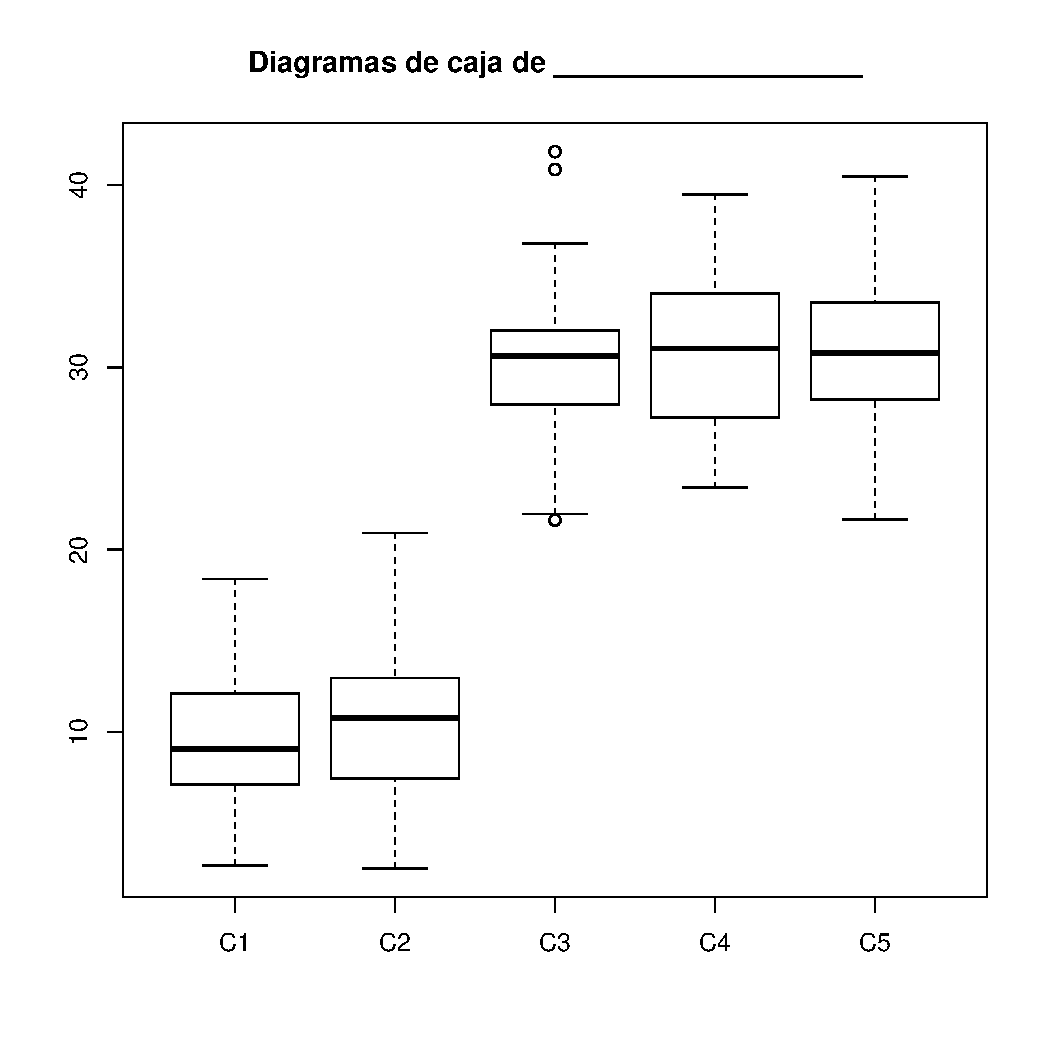
\includegraphics[width=\maxwidth]{figure/anova2-1} 

\end{knitrout}


Contestad a las siguientes cuestiones justificando que parte del código utilizáis

\punt  Interpretar y poner un título adecuado al diagrama de cajas ¿Qué nos dice el diagrama sobre la igualdad de medias del retraso? (\textbf{ 0.5 puntos})
\begin{knitrout}
\definecolor{shadecolor}{rgb}{0.969, 0.969, 0.969}\color{fgcolor}\begin{kframe}
\begin{alltt}
\hlkwd{boxplot}\hlstd{(datos_vuelos}\hlopt{$}\hlstd{retraso}\hlopt{~}\hlstd{datos_vuelos}\hlopt{$}\hlstd{compania,}
        \hlkwc{main}\hlstd{=}\hlstr{"Diagramas de caja de la variable retraso para cada compañía."}\hlstd{)}
\end{alltt}
\end{kframe}
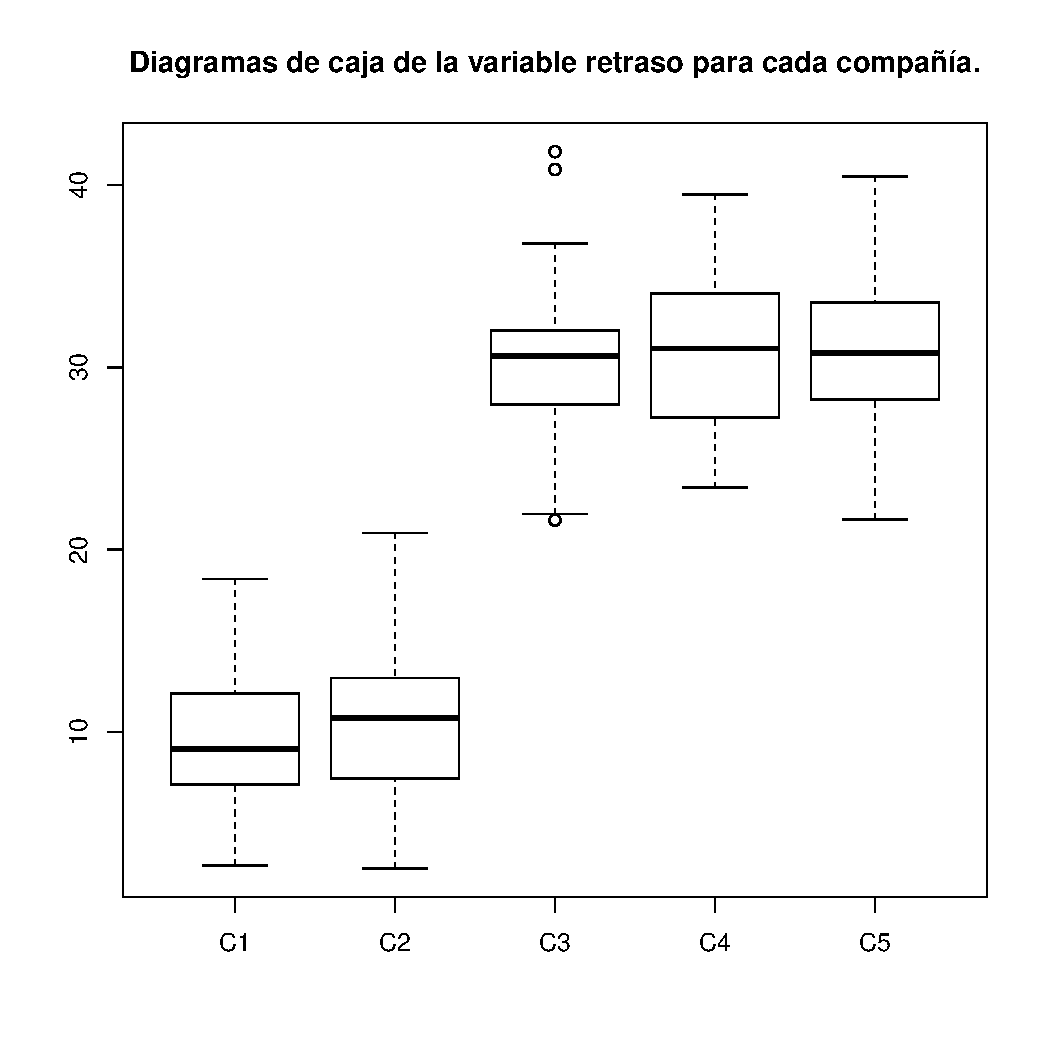
\includegraphics[width=\maxwidth]{figure/unnamed-chunk-1-1} 

\end{knitrout}

En este gráfico se muestran los diagramas de caja para cada una de las compañías.

Se observa que la dispersión medida gráficamente por la altura de la caja (diferencia ente el tercer y el primer cuartil) es semejante entre las ciudades, quizá la $C_4$ tiene mayor dispersión.

Respecto a la igualdad de medias por demos decir que las dos primeras compañías tienen retrasos menores y mediana menores que las compañías  $C_3,C_4,C_5,C_6$. Estas últimas compañía presentan diagramas de caja semejantes y medianas semejantes. Todo esto nos hace sospechar que las distribuciones de los retrasos de las  dos primeras compañías son similares y menores que las de las otras tres compañías que a su vez parecen tener 
distribuciones similares. 



\punt  Escribid hipótesis del contraste de ANOVA y discutid si se cumplen las condiciones necesarias para realizarlo. (\textbf{ 0.5 puntos})


Las condiciones del ANOVA de efectos fijos son una muestra aleatoria simple para cada nivel del factor, poblaciones normales  para la muestra de cada nivel del factor y de la misma varianza (homocedásticidad).

La condición del muestra alatoria simple viene dada por el diseño experimalntal del enunciado. La normalidad de las muestras para cada nivel del factor se comprueba con el test  de Lilliefors (con la función \verb+lillie+ de la librería \verb+nortest+), todos los $p$-valores son altos, el más pequeño es del 0rden de $0.07$ para el nivel $C_2$. Así que no hay evidencias fuertes para rechazar la normalidad de las distribuciones en cada  ciudad.

La igualdad de varianzas entre ciudades se resuleve con el test de Levene con la función \verb+levene.tes+ de la librería \verb+car+ el que se obtine un $p$-valor alto del orden de $0.984$ conformado por el test de homogeneidad de varianzas de Bartlett (función \verb+bartlett.test+ ) con un $p$-valor del orden  de $0.38$

Así que o hay evidencias fuertes en contra de la hocedasticidad y normalidad de cada muestra.


\punt  Escribid la tabla (estándar, la de los apuntes) del ANOVA con toda la información de qué es y cómo se calcula cada valor. Concluid en base a ello el resultado del ANOVA (\textbf{ 0.5 puntos})




\punt  Sea cual sea el resultado del ANOVA, realizad el ajuste por Bonferroni para $\alpha = 0.1$ y discutid los resultados obtenidos a partir la salida del  código. (\textbf{ 0.5 puntos})

\punt Discutid el resultado de la salida del código del test de Duncan. (\textbf{ 0.5 puntos})

\textbf{Solución:}

{\sc












}


\newpage

\probl  Para estudiar si hay evidencia de que el retraso de un vuelo en la salida aumenta el retraso de su llegada se toma una muestra aleatoria simple de 100 vuelos y se anota para cada vuelo si tuvo retraso en la salida y en la llegada (en minutos).
La tabla siguiente resume los resultados:





% <<tabla,echo=FALSE>>=
% library(knitr)
% cat(kable(aux,format="latex"))
% @

$$
\begin{tabular}{l|r|r}

\hline
Salida /Llegada  &  No Retraso  & Retraso\\
\hline
No Retraso & 75 & 15\\
\hline
Retraso & 6 & 4\\
\hline
\end{tabular}
$$



\punt Plantear un contraste de igualdad  de proporciones entre la proporción de vuelos  retrasados en la salida y en la llegada. ¿Qué diseño experimental estamos utilizando? (\textbf{0.5 puntos.})

\punt Resolver el contraste al nivel de significación $\alpha=0.1$ (\textbf{0.5 puntos.})

\punt Calcular el $p$-valor del contraste anterior. (\textbf{0.5 puntos.})

\punt Calcular e interpretar  un intervalo de confianza para la diferencia de proporciones al nivel 99\%. (\textbf{0.5 puntos.})


\begin{knitrout}
\definecolor{shadecolor}{rgb}{0.969, 0.969, 0.969}\color{fgcolor}\begin{kframe}
\begin{alltt}
\hlkwd{set.seed}\hlstd{(}\hlnum{2018}\hlstd{)}
\hlstd{salida} \hlkwb{=}\hlkwd{rbinom}\hlstd{(}\hlnum{100}\hlstd{,}\hlkwc{size}\hlstd{=}\hlnum{1}\hlstd{,}\hlkwc{prob}\hlstd{=}\hlnum{0.1}\hlstd{)}
\hlstd{llegada}\hlkwb{=}\hlkwd{rbinom}\hlstd{(}\hlnum{100}\hlstd{,}\hlkwc{size}\hlstd{=}\hlnum{1}\hlstd{,}\hlkwc{prob}\hlstd{=}\hlnum{0.2}\hlstd{)}
\hlstd{aux}\hlkwb{=}\hlkwd{table}\hlstd{(salida,llegada)}
\hlstd{b}\hlkwb{=}\hlstd{aux[}\hlnum{2}\hlstd{,}\hlnum{1}\hlstd{]}
\hlstd{b}
\end{alltt}
\begin{verbatim}
## [1] 6
\end{verbatim}
\begin{alltt}
\hlstd{d}\hlkwb{=}\hlstd{aux[}\hlnum{1}\hlstd{,}\hlnum{2}\hlstd{]}
\hlstd{d}
\end{alltt}
\begin{verbatim}
## [1] 15
\end{verbatim}
\begin{alltt}
\hlstd{n}\hlkwb{=}\hlkwd{sum}\hlstd{(aux)}
\hlstd{n}
\end{alltt}
\begin{verbatim}
## [1] 100
\end{verbatim}
\begin{alltt}
\hlstd{t}\hlkwb{=}\hlstd{(b}\hlopt{/}\hlstd{n}\hlopt{-}\hlstd{d}\hlopt{/}\hlstd{n)}\hlopt{/}\hlkwd{sqrt}\hlstd{((b}\hlopt{+}\hlstd{d)}\hlopt{/}\hlstd{n}\hlopt{^}\hlnum{2}\hlstd{)}
\hlstd{t}
\end{alltt}
\begin{verbatim}
## [1] -1.963961
\end{verbatim}
\begin{alltt}
\hlnum{2}\hlopt{*}\hlstd{(}\hlnum{1}\hlopt{-}\hlkwd{pt}\hlstd{(}\hlkwd{abs}\hlstd{(t),}\hlnum{100}\hlopt{-}\hlnum{1}\hlstd{))}
\end{alltt}
\begin{verbatim}
## [1] 0.05233902
\end{verbatim}
\begin{alltt}
\hlstd{t}\hlopt{^}\hlnum{2}
\end{alltt}
\begin{verbatim}
## [1] 3.857143
\end{verbatim}
\end{kframe}
\end{knitrout}


\begin{knitrout}
\definecolor{shadecolor}{rgb}{0.969, 0.969, 0.969}\color{fgcolor}\begin{kframe}
\begin{alltt}
\hlkwd{mcnemar.test}\hlstd{(aux,}\hlkwc{correct}\hlstd{=}\hlnum{FALSE}\hlstd{)}
\end{alltt}
\begin{verbatim}
## 
## 	McNemar's Chi-squared test
## 
## data:  aux
## McNemar's chi-squared = 3.8571, df = 1, p-value = 0.04953
\end{verbatim}
\begin{alltt}
\hlkwd{mcnemar.test}\hlstd{(aux,}\hlkwc{correct}\hlstd{=}\hlnum{FALSE}\hlstd{)}\hlopt{$}\hlstd{statistic}
\end{alltt}
\begin{verbatim}
## McNemar's chi-squared 
##              3.857143
\end{verbatim}
\end{kframe}
\end{knitrout}


\probl Se piensa que el tiempo en segundos transcurrido entre dos reservas de vuelos de avión  en un mismo día podría seguir una distribución exponencial con una reserva cada cinco segundos. Se  toma una muestra de 10 tiempos en segundos. 




% latex table generated in R 3.4.4 by xtable 1.8-2 package
% Thu Jun  7 11:32:07 2018
\begin{table}[ht]
\centering
\begin{tabular}{rrrrrrrrrrr}
  \hline
 Vuelo & 1 & 2 & 3 & 4 & 5 & 6 & 7 & 8 & 9 & 10 \\ 
  \hline
Retraso & 0.50 & 1.40 & 1.60 & 2.20 & 2.40 & 3.70 & 3.90 & 4.50 & 5.20 & 7.10 \\ 
   \hline
\end{tabular}
%\caption{latex} 
\end{table}


\punt ¿Cuál es y qué parámetros tiene la función de distribución teórica propuesta? Escribid correctamente la función de distribucion. (\textbf{0.5 puntos})

\punt   Contrastar la hipótesis del enunciado con el test KS, al nivel de significación $\alpha=0.1$. (\textbf{1 puntos})
\begin{knitrout}
\definecolor{shadecolor}{rgb}{0.969, 0.969, 0.969}\color{fgcolor}\begin{kframe}
\begin{alltt}
\hlkwd{set.seed}\hlstd{(}\hlnum{2018}\hlstd{)}
\hlstd{datos}\hlkwb{=}\hlkwd{sort}\hlstd{(}\hlkwd{round}\hlstd{(}\hlkwd{rexp}\hlstd{(}\hlnum{10}\hlstd{,}\hlnum{1}\hlopt{/}\hlnum{5}\hlstd{),}\hlnum{1}\hlstd{))}
\hlkwd{ks.test}\hlstd{(datos,}\hlstr{"pexp"}\hlstd{,}\hlnum{1}\hlopt{/}\hlnum{5}\hlstd{)}
\end{alltt}
\begin{verbatim}
## 
## 	One-sample Kolmogorov-Smirnov test
## 
## data:  datos
## D = 0.25345, p-value = 0.4669
## alternative hypothesis: two-sided
\end{verbatim}
\begin{alltt}
\hlstd{teoricas}\hlkwb{=}\hlkwd{pexp}\hlstd{(datos,}\hlnum{1}\hlopt{/}\hlnum{5}\hlstd{)}
\hlstd{teoricas}
\end{alltt}
\begin{verbatim}
##  [1] 0.09516258 0.24421626 0.27385096 0.35596358 0.38121661 0.52288608
##  [7] 0.54159399 0.59343034 0.64654532 0.75828598
\end{verbatim}
\begin{alltt}
\hlstd{obs}\hlkwb{=}\hlstd{(}\hlnum{1}\hlopt{:}\hlnum{10}\hlstd{)}\hlopt{/}\hlnum{10}
\hlstd{obs}
\end{alltt}
\begin{verbatim}
##  [1] 0.1 0.2 0.3 0.4 0.5 0.6 0.7 0.8 0.9 1.0
\end{verbatim}
\begin{alltt}
\hlkwd{abs}\hlstd{(teoricas}\hlopt{-} \hlstd{((}\hlnum{1}\hlopt{:}\hlnum{10}\hlstd{)}\hlopt{-}\hlnum{1}\hlstd{)}\hlopt{/}\hlnum{10}\hlstd{)}
\end{alltt}
\begin{verbatim}
##  [1] 0.09516258 0.14421626 0.07385096 0.05596358 0.01878339 0.02288608
##  [7] 0.05840601 0.10656966 0.15345468 0.14171402
\end{verbatim}
\begin{alltt}
\hlkwd{abs}\hlstd{(teoricas}\hlopt{-} \hlstd{(}\hlnum{1}\hlopt{:}\hlnum{10}\hlstd{)}\hlopt{/}\hlnum{10}\hlstd{)}
\end{alltt}
\begin{verbatim}
##  [1] 0.004837418 0.044216259 0.026149037 0.044036421 0.118783392
##  [6] 0.077113916 0.158406011 0.206569660 0.253454682 0.241714017
\end{verbatim}
\begin{alltt}
\hlstd{D}\hlkwb{=}\hlkwd{pmax}\hlstd{(}\hlkwd{abs}\hlstd{(teoricas}\hlopt{-} \hlstd{((}\hlnum{1}\hlopt{:}\hlnum{10}\hlstd{)}\hlopt{-}\hlnum{1}\hlstd{)}\hlopt{/}\hlnum{10}\hlstd{),}\hlkwd{abs}\hlstd{(teoricas}\hlopt{-} \hlstd{(}\hlnum{1}\hlopt{:}\hlnum{10}\hlstd{)}\hlopt{/}\hlnum{10}\hlstd{))}
\hlstd{D}
\end{alltt}
\begin{verbatim}
##  [1] 0.09516258 0.14421626 0.07385096 0.05596358 0.11878339 0.07711392
##  [7] 0.15840601 0.20656966 0.25345468 0.24171402
\end{verbatim}
\begin{alltt}
\hlkwd{max}\hlstd{(D)}
\end{alltt}
\begin{verbatim}
## [1] 0.2534547
\end{verbatim}
\end{kframe}
\end{knitrout}

\probl La siguiente tabla contiene los valores de \verb+retraso_llegada, retraso_salida+ y \verb+distancia+ del trayecto del vuelo para cuatro vuelos. Las distancias vienen dadas en centenas de kilómetros y los retrasos en decenas de minutos. 



\begin{knitrout}
\definecolor{shadecolor}{rgb}{0.969, 0.969, 0.969}\color{fgcolor}\begin{kframe}
\begin{alltt}
\hlstd{df}\hlkwb{=}\hlkwd{data.frame}\hlstd{(retraso_llegada,retraso_salida,distancia)}
\hlstd{df}
\end{alltt}
\begin{verbatim}
##   retraso_llegada retraso_salida distancia
## 1              27              3        10
## 2              -9             -1        15
## 3              18              2        20
## 4              46              5         5
\end{verbatim}
\begin{alltt}
\hlstd{X}\hlkwb{=}\hlkwd{cbind}\hlstd{(}\hlkwd{rep}\hlstd{(}\hlnum{1}\hlstd{,}\hlnum{4}\hlstd{),df}\hlopt{$}\hlstd{retraso_salida,df}\hlopt{$}\hlstd{distancia)}
\hlstd{X}
\end{alltt}
\begin{verbatim}
##      [,1] [,2] [,3]
## [1,]    1    3   10
## [2,]    1   -1   15
## [3,]    1    2   20
## [4,]    1    5    5
\end{verbatim}
\begin{alltt}
\hlstd{Y}\hlkwb{=}\hlkwd{matrix}\hlstd{(df}\hlopt{$}\hlstd{retraso_llegada,}\hlkwc{ncol}\hlstd{=}\hlnum{1}\hlstd{)}
\hlstd{Y}
\end{alltt}
\begin{verbatim}
##      [,1]
## [1,]   27
## [2,]   -9
## [3,]   18
## [4,]   46
\end{verbatim}
\begin{alltt}
\hlkwd{t}\hlstd{(X)}\hlopt\hlstd{X}
\end{alltt}
\begin{verbatim}
##      [,1] [,2] [,3]
## [1,]    4    9   50
## [2,]    9   39   80
## [3,]   50   80  750
\end{verbatim}
\begin{alltt}
\hlkwd{det}\hlstd{(}\hlkwd{t}\hlstd{(X)}\hlopt\hlstd{X)}
\end{alltt}
\begin{verbatim}
## [1] 5150
\end{verbatim}
\begin{alltt}
\hlkwd{solve}\hlstd{(}\hlkwd{t}\hlstd{(X)}\hlopt\hlstd{X)}
\end{alltt}
\begin{verbatim}
##            [,1]        [,2]        [,3]
## [1,]  4.4368932 -0.53398058 -0.23883495
## [2,] -0.5339806  0.09708738  0.02524272
## [3,] -0.2388350  0.02524272  0.01456311
\end{verbatim}
\begin{alltt}
\hlkwd{solve}\hlstd{(}\hlkwd{t}\hlstd{(X)}\hlopt\hlstd{X)}\hlopt\hlkwd{t}\hlstd{(X)}\hlopt\hlstd{Y}
\end{alltt}
\begin{verbatim}
##             [,1]
## [1,]  0.57281553
## [2,]  9.07766990
## [3,] -0.03980583
\end{verbatim}
\begin{alltt}
\hlstd{X}\hlopt\hlkwd{solve}\hlstd{(}\hlkwd{t}\hlstd{(X)}\hlopt\hlstd{X)}\hlopt\hlkwd{t}\hlstd{(X)}\hlopt\hlstd{Y}
\end{alltt}
\begin{verbatim}
##           [,1]
## [1,] 27.407767
## [2,] -9.101942
## [3,] 17.932039
## [4,] 45.762136
\end{verbatim}
\begin{alltt}
\hlkwd{sum}\hlstd{((X}\hlopt\hlkwd{solve}\hlstd{(}\hlkwd{t}\hlstd{(X)}\hlopt\hlstd{X)}\hlopt\hlkwd{t}\hlstd{(X)}\hlopt\hlstd{Y)}\hlopt{^}\hlnum{2}\hlstd{)}
\end{alltt}
\begin{verbatim}
## [1] 3249.762
\end{verbatim}
\end{kframe}
\end{knitrout}


   
Usad el código anterior cuando pertoque para contestar a las siguientes preguntas.

\punt Escribid y explicad la ecuación del modelo de regresión lineal múltiple que predice el \verb+retraso_llegada+ a partir de las otras dos variables. (\textbf{0.5 puntos.})

\punt Calcular $R^2$ y $R^2$ ajustado de la anterior regresión. (\textbf{0.5 puntos.}) 

\begin{knitrout}
\definecolor{shadecolor}{rgb}{0.969, 0.969, 0.969}\color{fgcolor}\begin{kframe}
\begin{alltt}
\hlstd{sumYhat_square}\hlkwb{=}\hlkwd{sum}\hlstd{((X}\hlopt\hlkwd{solve}\hlstd{(}\hlkwd{t}\hlstd{(X)}\hlopt\hlstd{X)}\hlopt\hlkwd{t}\hlstd{(X)}\hlopt\hlstd{Y)}\hlopt{^}\hlnum{2}\hlstd{)}\hlcom{# ya se daba}
\hlstd{meanY}\hlkwb{=}\hlkwd{mean}\hlstd{(Y)}\hlcom{# a mano}
\hlstd{SST}\hlkwb{=}\hlnum{4}\hlopt{*}\hlstd{(}\hlkwd{sum}\hlstd{(Y}\hlopt{^}\hlnum{2}\hlstd{)}\hlopt{/}\hlnum{4}\hlopt{-}\hlkwd{mean}\hlstd{(Y)}\hlopt{^}\hlnum{2}\hlstd{)}\hlcom{#a mano}
\hlstd{SST}
\end{alltt}
\begin{verbatim}
## [1] 1569
\end{verbatim}
\begin{alltt}
\hlstd{Error}\hlkwb{=}\hlstd{Y}\hlopt{-}\hlstd{X}\hlopt\hlkwd{solve}\hlstd{(}\hlkwd{t}\hlstd{(X)}\hlopt\hlstd{X)}\hlopt\hlkwd{t}\hlstd{(X)}\hlopt\hlstd{Y}
\hlstd{SSR}\hlkwb{=}\hlnum{4}\hlopt{*}\hlstd{(sumYhat_square}\hlopt{/}\hlnum{4}\hlopt{-}\hlstd{meanY}\hlopt{^}\hlnum{2}\hlstd{)}
\hlstd{SSR}
\end{alltt}
\begin{verbatim}
## [1] 1568.762
\end{verbatim}
\begin{alltt}
\hlstd{R2}\hlkwb{=}\hlstd{SSR}\hlopt{/}\hlstd{SST}
\hlstd{R2}
\end{alltt}
\begin{verbatim}
## [1] 0.9998484
\end{verbatim}
\begin{alltt}
\hlkwd{summary}\hlstd{(sol)}\hlopt{$}\hlstd{r.squared}
\end{alltt}
\begin{verbatim}
## [1] 0.9998484
\end{verbatim}
\begin{alltt}
\hlstd{R2adj}\hlkwb{=}\hlnum{1}\hlopt{-}\hlstd{(}\hlnum{1}\hlopt{-}\hlstd{R2)}\hlopt{*}\hlstd{(}\hlnum{4}\hlopt{-}\hlnum{1}\hlstd{)}\hlopt{/}\hlstd{(}\hlnum{4}\hlopt{-}\hlnum{2}\hlopt{-}\hlnum{1}\hlstd{)}
\hlstd{R2adj}
\end{alltt}
\begin{verbatim}
## [1] 0.9995452
\end{verbatim}
\begin{alltt}
\hlkwd{summary}\hlstd{(sol)}\hlopt{$}\hlstd{adj.r.squared}
\end{alltt}
\begin{verbatim}
## [1] 0.9995452
\end{verbatim}
\end{kframe}
\end{knitrout}

\punt  Calcula el AIC de este modelo. (\textbf{0.5 puntos.})


\begin{knitrout}
\definecolor{shadecolor}{rgb}{0.969, 0.969, 0.969}\color{fgcolor}\begin{kframe}
\begin{alltt}
\hlstd{SSE}\hlkwb{=}\hlstd{SST}\hlopt{-}\hlstd{SSR}
\hlstd{SSE}
\end{alltt}
\begin{verbatim}
## [1] 0.2378641
\end{verbatim}
\begin{alltt}
\hlstd{AIC_value}\hlkwb{=}\hlnum{4}\hlopt{*}\hlkwd{log}\hlstd{(SSE}\hlopt{/}\hlnum{4}\hlstd{)}\hlopt{+}\hlnum{2}\hlopt{*}\hlnum{2}
\hlstd{AIC_value}
\end{alltt}
\begin{verbatim}
## [1] -7.289401
\end{verbatim}
\end{kframe}
\end{knitrout}
\punt Calcular el intervalo de confianza al 95\% para el  coeficiente de la variable distancia ¿Qué se puede deducir de su presencia en el modelo? (\textbf{0.5 puntos.})

\begin{knitrout}
\definecolor{shadecolor}{rgb}{0.969, 0.969, 0.969}\color{fgcolor}\begin{kframe}
\begin{alltt}
\hlkwd{confint}\hlstd{(sol)}
\end{alltt}
\begin{verbatim}
##                      2.5 %     97.5 %
## (Intercept)    -12.4804678 13.6260989
## retraso_salida   7.1467615 11.0085783
## distancia       -0.7876434  0.7080318
\end{verbatim}
\end{kframe}
\end{knitrout}


\begin{knitrout}
\definecolor{shadecolor}{rgb}{0.969, 0.969, 0.969}\color{fgcolor}\begin{kframe}
\begin{alltt}
\hlstd{sol}\hlopt{$}\hlstd{coefficients[}\hlnum{3}\hlstd{]}\hlopt{+}\hlkwd{c}\hlstd{(}\hlopt{-}\hlnum{1}\hlstd{,}\hlnum{1}\hlstd{)}\hlopt{*}\hlkwd{qt}\hlstd{(}\hlnum{0.975}\hlstd{,}\hlnum{4}\hlopt{-}\hlnum{2}\hlopt{-}\hlnum{1}\hlstd{)}\hlopt{*}
  \hlkwd{sqrt}\hlstd{(SSE}\hlopt{/}\hlstd{(}\hlnum{4}\hlopt{-}\hlnum{2}\hlopt{-}\hlnum{1}\hlstd{)}\hlopt{*}\hlkwd{solve}\hlstd{(}\hlkwd{t}\hlstd{(X)}\hlopt\hlstd{X)[}\hlnum{3}\hlstd{,}\hlnum{3}\hlstd{])}
\end{alltt}
\begin{verbatim}
## [1] -0.7876434  0.7080318
\end{verbatim}
\end{kframe}
\end{knitrout}

\end{document}

